
La dernière alerte modélisée est le cas dit du \enquote{fil rouge} que
nous avions présenté dans le premier chapitre de cette thèse. Comme
nous l'avions indiqué lors de sa première présentation, le \emph{fil
  rouge} est une alerte particulière, contenant de nombreux indices
très imprécis et incertains. Par conséquent la \ac{zir} est
extrêmement étendue.


\subsection{Présentation de l'alerte}
\label{subsec:9-4-1}

Le fil rouge est une alerte composée de XX \emph{indices de
  localisation.}


Faute d'enregistrement audio, le fil rouge n'a pas été retranscrit,
les indices dont nous disposons (et qui avaient été présentés dans le
\autoref{chap:01}) ont donc été directement saisis par le secouriste.
%
de ce fait, le \emph{fil rouge} est une alerte assez différente des
précédentes, puisque XXX n'est pas
%
Le traitement du \emph{fil rouge} est donc plus proche du traitement
opérationnel qui sera réellement effectué lors du traitement d'une
alerte.


Pour le cas du \emph{fil rouge} nous ne disposons pas de
l'enregistrement audio et donc de son verbatim, les indices ayant déjà 
été synthétisés par les secouristes. Les les avions déjà présentés
dans le \autoref{chap:01}.
%
Pour rappel voici la synthèse de l'alerte qui nous a été donnée par
les secouristes :
%
\begin{enumerate}
\item La victime est partie de \emph{Bourg-d'Oisans,} à pied, sur
  chemin, en direction d'une station de ski.
\item La victime a marché plusieurs heures.
\item La victime a chuté de plusieurs mètres.
\item La victime voit une partie de plan d'eau.
\item La victime est sous une route et entend des véhicules.
\item La victime est sous une ligne électrique 3 brins.
\item La victime vient de passer du soleil à l'ombre.
\item Le téléphone de la victime est connecté à une antenne GSM située
  à la chapelle \emph{St-Philomene} à \emph{Villard-Reymond} et
  orientée à \SI{90}{\degree}
\end{enumerate}

Comme nous l'avions déjà signalé lors de la présentation du \emph{fil
  rouge} (\autoref{chap:01}), ces différentes informations sont
fortement imprécises, surtout si on les compare aux extraits des
alertes \emph{Grand Veymont} (\autoref{anx:retrans_grand_veymont}) et
\emph{Moucherotte} (\autoref{anx:retrans_moucherotte}). Les
descriptions sont ici peu informatives et discriminantes et la
construction d'indices de localisations est par conséquent plus
délicate.

La première de ces sept descriptions donne plusieurs informations sur
le trajet suivit par la victime jusqu'à sa position actuelle. Elle
nous renseigne sur son point de départ, clairement identifié, sa
destination visée, une station de ski inconnue et son mode de
déplacement, à pied sur un chemin. Ces informations ne sont cependant
pas directement transposables en un indice de localisation. On
pourrait certes supposer qu'étant donné que \enquote{La victime est
  partie de \emph{Bourg-d'Oisans}}, elle est probablement à proximité
de cette ville, ce qui permettrait d'utiliser les relations de
localisations \onto[orl]{Aux\-Alentours\-De} ou
\onto[orl]{Proximal}. Cependant, rien dans cette première description
ne nous permet d'affirmer que la victime est toujours à proximité de
\emph{Bourg-d'Oisans.} En effet, nous ne connaissons pas la durée de
sa sortie et il se peut que la victime ait parcouru suffisamment de
kilomètres pour que ces relations de localisaiton ne soient plus
valides. Il nous semble donc prématuré d'utiliser ces relations de
localisaiton. De manière similaire nous pourrions envisager d'utiliser
la relation de localisation
\onto[orla]{Si\-tue\-Sur\-Itineraire\-Ou\-Reseau\-Support}, la victime
ayant indiqué avoir utilisé un chemin. Cependant, les expressions
suivantes nous indiquent que la victime \enquote{a chuté de plusieurs
  mètres}. Il est par conséquent difficile d'affirmer que la victime
se situe toujours sur un chemin, c'est pourquoi il ne nous semble pas
pertinent d'utiliser cette relation de localisaiton. Il est cependant
possible de construire un indice de localisation à partir de cette
première description. En effet, la victime indique qu'elle est partie
de \emph{Bourg-d'Oisans} dans la direction \enquote{globale} d'une
station de ski, ce qui nous renseigne sur sa direction globale. Or, la
relation de localisation
\onto[orl]{Dans\-La\-Direction\-De\-X\-Depuis\-Y} a été conçue pour
modéliser ce type d'informations, sans préjuger du mode ou du support
de déplacement.

Le second élément de cette alerte, \enquote{La victime a marché
  plusieurs heures}, donne un premier complément d'informations aux
informations précédentes. Grâce à la connaissance du point de départ
et à l'identification du temps de déplacement, nous pouvons construire
une estimation de la distance parcourue par la victime. Pour ce faire
nous avons défini une relation de localisation
\onto[orl]{A\-Temps\-De\-Marche\-De}, permettant de construire la
\ac{zlc} atteignable en un temps de marche et à partir d'un point de
départ donné. La possibilité de construire un tel indice de
localisation remplace avantageusement l'utilisation d'une relation de
localisation telle que \onto[orl]{Aux\-Alentours\-De}. En effet, cette
dernière ne donne qu'une information très vague sur la zone de
présence de la victime, alors que la relation de localisation
\onto[orl]{A\-Temps\-De\-Marche\-De} permet une modélisation plus
fine, même dans le cas présent, où l'estimation du temps de parcours
est très imprécise. Dans le cas de cette alerte nous avons donc
considéré qu'il était inutile de définir un indice de localisation
employant les relations de localisaiton \onto[orl]{Aux\-Alentours\-De}
ou \onto[orl]{Proximal}, la relation
\onto[orl]{A\-Temps\-De\-Marche\-De} quantifiant également un
éloignement au point de départ, mais de manière plus discriminante.

Le troisième élément de l'alerte nous indique que \enquote{la victime
  a chuté de plusieurs mètres}. Prise sous cette forme, cette
description n'est pas interprétable comme un indice de localisation et
aucune des relations que nous avons définies ne permet de
l'exprimer. Il est cependant possible de combiner cette information
avec les descriptions précédentes, de manière à construire un nouvel
indice de localisation. Ces descriptions nous renseignent, en effet,
sur le potentiel contexte de cette chute. Comme la victime a indiqué
qu'elle se déplaçait à pied, sur un chemin, nous pouvons supposer que
c'était également le cas lors de sa chute. Nous pouvons alors en
déduire que, suite à sa chute, la victime se situe sous un
chemin. Cette information extrapolée peut ainsi être modélisée avec la
relation de localisation \onto[orl]{Sous\-Altitude} ou l'une des
relations qui en dérivent. Compte-tenu du contexte de la chute, la
relation de localisation plus appropriée nous semble être
\onto[orl]{Sous\-Proche\-De}, puisqu’elle ajoute une contrainte de
proximité planimétrique. Ainsi s'il nous est impossible de construire
directement une \ac{zlc} grâce à l'information \enquote{J'ai chuté de
  plusieurs mètres}, il nous est en revanche possible de dériver de
cette information un indice de localisation exprimant la position
actuelle de la victime, par rapport au chemin dont elle vient de
chuter.

L'interprétation de la quatrième description de l'alerte, \enquote{La
  victime voit une partie d'un plan d'eau}, est plus évidente que
celle des descriptions précédentes. En effet, deux relations de
localisation spécifiques ont été introduites pour traiter des
relations de visibilité \onto[orl]{Site\-Voit\-Cible} et
\onto[orl]{Cible\-Voit\-Site}. Ces différentes relations permettent de
distinguer les visibilités actives et passives. Dans le cas présent,
la victime décrit ce qu'elle voit, on est donc dans une situation
modélisable à l'aide de la relation de localisation
\onto[orl]{Cible\-Voit\-Site}. Cette description présente cependant la
particularité d'employer l’adverbe \enquote{presque} précisant que le
plan d'eau mentionné n'est pas vu dans son intégralité. Dans sa
configuration initiale la relation \onto[orl]{Cible\-Voit\-Site} ne
permet pas d'exprimer une telle description, il est donc nécessaire
d'employer un modifieur, ce que nous détaillerons lors de la
modélisation de cet indice de localisation.

De manière similaire, la cinquième description, \enquote{La victime
  est sous une route et entend des voitures}, est assez explicite. On
reconnait dans cette formulation l'utilisation de la préposition
\enquote{sous} traduisant une relation de verticalité. Or, comme nous
l'indiquions lors de l'analyse de la seconde description (\enquote{La
  victime a chuté de plusieurs mètres}), la relation de localisation
\onto{Sous\-Altitude}, n'apportant aucune contrainte sur l'axe
horizontal, n'est pas nécessairement la plus pertinente ici. On peut
donc utiliser une nouvelle fois la relation de localisation
\onto[orl]{Sous\-Proche\-De} pour construire un nouvel indice de
localisation. Cette description donne une seconde information,
\enquote{la victime entend des véhicules}. Cette dernière n'est, une
nouvelle, pas directement interprétable avec une relation de
localisation, pourtant cette information peut être exploitée de
manière à raffiner la modélisation de \emph{l'indice de localisation.}
On peut tirer deux informations différentes de cette indication. Tout
d'abord une indication de proximité. En effet, la victime indique
indirectement qu'elle se situe a portée de son de la route, ce qui, si
l'on disposait d'un modèle adapté, permettrait d'estimer la distance
de victime à la route.Il serait même possible de définir une nouvelle
relation de localisation \onto{A\-Porte\-De\-Son} pour retranscrire
cette indication. Une telle relation permettrait sans aucun doute
d'affiner cette approximation, particulièrement si elle permet la
prise en compte des effets d’échos, particulièrement présents en
montagne, pouvant conduire à une perception faussée de la distance
d'un son. Cependant nous n'avons pas travaillé au développement d'une
telle méthode, cette alerte étant la seule où une portée sonore est
mentionnée. La seconde information que l'on peut tirer de cet élément
est la nature de la route. On peut en effet considérer que, pour que
la victime note entendre une route, il est nécessaire que celle-ci
soit suffisamment fréquentée pour que le trafic soit notable. Un tel
critère permet d'affiner la sélection des objets de référence, qui,
compte-tenu de l’imprécision de la description, seront relativement
nombreux. Il est cependant délicat de procéder à une telle sélection
sans risquer de supprimer des objets de référence pertinents, et donc
de créer des faux négatifs. En effet, l'hypothèse que nous proposons
ici est assez contraignante et il nous semble inenvisageable de
l'appliquer sans la confirmation de la victime.

Dans la sixième description, la victime indique qu'elle se situe sous
une ligne électrique trois brins. Nous avons déjà présenté ce cas,
notamment dans le \autoref{chap:06} où nous comparions les différentes
implémentations de la théorie des sous-ensembles flous pour
représenter des zones de localisation. Si nous n'avions pas encore
présenté les différentes relations de localisation, définies dans
l'ontologie des relations de localisation, nous avions déjà expliqué
que cette description nécessitait que la relation de verticalité entre
le \emph{site} et la \emph{cible} soit contrainte selon l'axe
horizontal. Dit autrement, il est ici nécessaire d'être proche du
\emph{site} et à une altitude inférieure du \emph{site} pour que l'on
puisse affirmer qu'une position soit \enquote{sous} le \emph{site.}
La relation de localisation \onto{Sous\-Proche\-De} a spécifiquement
été définie pour modéliser ce type de relation.

La septième description donnée par le secouriste nous indique que la
position de la victime vient de passer du Soleil à l'ombre. Une
nouvelle fois nous n'avons pas défini de relation de localisation
permettant de modéliser un tel indice, celui-ci n'apparaissant qu'une
seule fois dans l'ensemble du corpus d'alertes. Il serait cependant
possible de mettre en place une telle relation de localisation,
plusieurs bibliothèques permettant de modéliser les ombres produites
par le relief en fonction de l'heure de la journée.

La huitième et dernière information que nous ayons sur cette alerte
donne la position du relais téléphonique auquel le téléphone de la
victime est connecté. Comme pour la description précédente nous
n'avons pas défini une relation de localisation spécifique à ce type
d'information, mais pour des raisons différentes. En effet, si
l’indication \enquote{Je viens de passer du Soleil à l'ombre} est
unique, ce qui nous a conduit à l'ignorer provisoirement, la
connaissance de l'antenne de rattachement du téléphone de la victime
est plus fréquente. Toutefois l'exploitation fine de cet indice est
assez complexe, comme nous l'avions rapidement évoqué dans le
\autoref{chap:01}. L'implémentation d'une hypothétique relation
\onto{Connecte\-A\-Antenne} nécessiterai, en effet, de prendre la
portée du signal, fortement influencée par les conditions
climatiques. Nous avons donc choisi d'ajourner sa définition. Il est
cependant possible d'utiliser cette information pour extrapoler un
nouvel indice de localisation, certes moins précis que celui que l'on
pourrait obtenir avec une relation de localisation dédiée, mais tout
de même discriminant. On connait en effet l'orientation générale de
l'antenne téléphonique de à laquelle le téléphone de la victime est
connecté. On peut alors approximer la zone où le téléphone de la
victime peut se connecter à une antenne donnée en l'approximant à
l'aide d'une relation cardinale. On peut ici employer la relation de
localisation \onto[orl]{A\-L\-Est\-De}, pour créer ce cône. Il n'y a
ici pas de raisons d'employer une des relations de localisation
dérivée de \onto[orl]{A\-L\-Est\-De}, comme
\onto[orl]{Dans\-La\-Partie\-Est\-De} ou
\onto[orl]{A\-L\-Est\-De\-Externe}. En effet, l'objet de référence
utilisé pour cet indice de localisation, une antenne GSM, n'est pas de
taille suffisante pour que cette distinction est un sens. Cette
approche ne permettra cependant pas de modéliser la portée du signal,
le cône construit par la relation \onto[orl]{A\-L\-Est\-De} étant
virtuellement infini. Cette approximation dans la modélisation de ce
dernier indice est certes insatisfaisante en soi, mais elle devient
parfaitement acceptable lorsque remise dans le contexte de la
modélisation de l'alerte dans son ensemble, la multiplication des
indices de localisation permettant de compenser la faiblesse de
certains d'entre eux.

Au terme de l'analyse de l'alerte on dispose donc de 7 indices de
localisation à spatialiser:
% 
\begin{enumerate}
\item \label{ind:fr1} La victime est
  \onto[orl]{Dans\-La\-Direction\-De\-X\-Depuis\-Y}
  \emph{Bourg-d'Oisans} (\texttt{X}) et une station de ski
  (\texttt{Y})
  % 
\item \label{ind:fr2} La victime est
  \onto[orl]{A\-Temps\-De\-Marche\-De} \emph{Bourg-d'Oisans} 
  % 
\item \label{ind:fr3} La victime est \onto[orl]{Sous\-Proche\-De} un
  chemin
  % 
\item \label{ind:fr4} La victime voit (\onto[orl]{Cible\-Voit\-Site})
  une partie d'un plan d'eau
  % 
\item \label{ind:fr5} La victime est \onto[orl]{Sous\-Proche\-De} une
  route
  % 
\item \label{ind:fr6} La victime est \onto[orl]{Sous\-Proche\-De} une
  ligne électrique trois brins
  % 
\item \label{ind:fr7} La victime est \onto[orl]{A\-L\-Est\-De}
  l'antenne GSM de la \emph{St-Philomene}, orientée à \SI{90}{\degree}
\end{enumerate}

\subsection{Modélisation de l'alerte}
\label{subsec:9-4-2}

La \ac{zir} définie pour cette alerte est une zone de
\SI{625}{\kilo\meter\squared}

\begin{figure}
  \centering
  \begin{tikzpicture}
  \tikzset{et/.style={above,font=\footnotesize\vphantom{Ag}}}
  % 
  \node[inner sep=0pt, anchor=south west] (image) at (0,0){\includegraphics{./figures/ZIR_fil_rouge.png}};
  % 
  \begin{scope}
    \node (P2) at ([yshift=-.5cm]image.south east) {};
    \node (P1) at ([yshift=-.5cm]image.south west) {};
    % 
    \node (rect) [anchor=north west, minimum width=1cm,minimum
    height=.25cm] at ([yshift=-.25cm]P1) {}; \path[draw=RdBu-9-1, line
    width=1mm](rect.west) --([xshift=-1ex]rect.south) -- ([xshift=1ex]rect.north)
    -- (rect.east);
    % 
    \node[anchor=west, font=\tiny\vphantom{Ag}, text width = 4cm] at
    ([xshift=1ex]rect.east) {Limite de la \ac{zir}};
    % Échelle
    % Échelle
    \draw[-] (P2 |- -1cm,-1cm) --++ (-1,0) node[et,pos=.5] {\SI{2,5}{\kilo\meter}};
    % Légende détaillée
    \path (P1) -- (P2) node[pos=.5, yshift=-1cm] {\tiny Pour la légende détaillée du fond topographique voir \autoref{anx:topo_leg}. Sources: BD TOPO 2018, BD ALTI 2018.}; 
  \end{scope}
\end{tikzpicture}
  \caption{Zone initiale de recherche pour le \emph{fil rouge}}
  \label{fig:zir_fil_rouge}
\end{figure}

% Direction
Le premier des indices de localisation de cette alerte (\ref{ind:fr1})
est fondé sur la relation de localisation
\onto[orl]{Dans\-La\-Direction\-De\-X\-Depuis\-Y}. Comme nous
l'expliquions précédent, cette relation de localisation permet de
modéliser une relation de direction sans considération de
l’implantation.
%
Cette relation de localisation est atomique et elle fait appel 


et un objet
géographique non nommé (\enquote{une station de ski}) comme objet de
référence.

\begin{figure}
  \centering
  \begin{tikzpicture} 
  \node[anchor=east,text width=3.5cm] (x1) at (-3.5,0) {\onto[orla]{Dans\-La\-Direction\-De\-X\-Depuis\-Y}};

  \node[anchor=west] (y1) at (3.5,.8) {\onto[orla]{Centroide}};
  \node[anchor=west] (y2) at (3.5,0) {\onto[orla]{Direction\-De}};
  \node[anchor=west] (y3) at (3.5,-0.8) {\onto[orla]{Inf\-Val\-0}};
  
  \fill[RdBu-9-9] (x1.east) circle (2pt);
  
  \fill[RdBu-9-1] (y1.west) circle (2pt);
  \fill[RdBu-9-1] (y2.west) circle (2pt);
  \fill[RdBu-9-1] (y3.west) circle (2pt);

  \draw[->, shorten >=5pt, shorten <=5pt] (x1.east) |- (y1.west)
  node[pos=0.75, sloped, anchor=center, fill=white] {\tiny\emph{À pour rasteriser}};
  
  \draw[->, shorten >=5pt, shorten <=5pt] (x1.east) -- (y2.west)
  node[pos=0.5, sloped, anchor=center, fill=white] {\tiny\emph{À pour métrique}};

    \draw[->, shorten >=5pt, shorten <=5pt] (x1.east) |- (y3.west)
  node[pos=0.75, sloped, anchor=center, fill=white] {\tiny\emph{À pour fuzzyficateur}};
\end{tikzpicture}
  \caption{Rasteriser, métrique et fuzzyficateur utilisés pour la
    spatialisation de la relation de localisation atomique
    \protect\onto[orla]{Dans\-La\-Direction\-De\-X\-Depuis\-Y}}
  \label{fig:ex_parties_statialisation_DanslaDirectionDe}
\end{figure}

L'utilisation d'un tel objet de référence nous contraints à procéder à
la décomposition de l'indice de localisation en fonction des
différentes instances correspondant à la description de l'objet de
référence. Dans le cas présent on peut identifier X stations de ski
dans la \ac{zir}, chacune entre elles pouvant être un objet de
référence potentiel.

La métrique, \onto[orla]{Direction\-De}, utilisée par cette relation
de localisation atomique 

% Temps de marche

Le second indice de localisaiton (\ref{ind:fr2}) emploie la relation
de localisation \onto[orl]{A\-Temps\-De\-Marche\-De}. Il s'agit une
nouvelle fois d'une relation de localisaiton atomique, qu'il n'est pas
nécessaire de décomposer. De même, l'objet de référence utilisé,
\emph{Bourg-d'Oisans} est nommé, il n'est donc pas nécessaire de
procéder à la décomposition des objets de référence.

Dans sa version \enquote{standart} la relation de localisation
atomique \onto[orla]{A\-Temps\-De\-Marche\-De} utilise le rasteriser
\onto[orla]{Geometrie}, la métrique \onto[orla]{} et la fuzzyficateur
\onto[orla]{Eq\-Val} prenant comme paramètre la durée de
déplacement. Toutefois le cas que nous modélisons ici est un peu
différent, puisque la durée donnée, \enquote{plusieurs heures}, est
très approximée.
%
L'utilisation du fuzzyficateur \onto[orla]{Eq\-Val}
n'est donc pas des plus adaptées.
%
Pour modéliser cet indice de localisation nous avons donc mis en place
une version \emph{ad hoc} de la relation de localisation
\onto[orla]{A\-Temps\-De\-Marche\-De} utilisant le fuzzyficateur
\onto[orla]{Sup\-Val}.

Cependant le changement du fuzzyficateur ne permet pas de XXX
%
Pour ce faire on peut ajouter un second indice, utilisant la même
relation de localisation, \onto[orla]{A\-Temps\-De\-Marche\-De}, mais
destinée à limiter la distance parcourue par la victime.
%


%\subsubsection{La victime est \protect\onto[orl]{Sous\-Proche\-De} un chemin}

L'indice de localisation suivant (\ref{ind:fr3}) utilise la relation
de localisation \onto[orl]{Sous\-Proche\-De} que nous avions déjà
présenté, sans la nommer, dans le \autoref{chap:06}. Cette relation de
localisation n'est pas atomique, elle est définie comme la conjonction
de deux relations de localisation atomiques,
\onto[orla]{Sous\-Altitude} et \onto[orla]{Proximal}.

La première de ces deux relations de localisation atomiques
\onto[orla]{Sous\-Altitude} a déjà été employée dans les exemples
précédents, comme pour la spatialisation de l'indice de localisaiton :
\enquote{Le requérant est \onto[orl]{Sous\-Altitude} du sommet du
  \emph{Grand Veymont}} (\ref{ind:gv2}) pour l'alerte :
\enquote{\emph{Grand Veymont}}. Pour rappel, cette relation de
localisation atomique emploie \onto[orla]{Geometrie} comme rasteriser,
\onto[orla]{Delta\-Nearest\-Val} comme métrique et
\onto[orla]{Inf\-Val\-0} comme fuzzyficateur
(\autoref{fig:ex_parties_statialisation_sousalt}).

Le seconde relation de localisaiton atomique, \onto[orla]{Proximal},


\begin{figure}
  \centering
  \begin{tikzpicture}
  \tikzset{et/.style={above,font=\footnotesize\vphantom{Ag}}}
  % 
  \node[inner sep=0pt, anchor=south west] (image) at (0,0){\includegraphics{./figures/ZIR_fil_rouge.png}};
  % 
  \begin{scope}
    \node (P2) at ([yshift=-.5cm]image.south east) {};
    \node (P1) at ([yshift=-.5cm]image.south west) {};
    % 
    \node (rect) [anchor=north west, minimum width=1cm,minimum
    height=.25cm] at ([yshift=-.25cm]P1) {}; \path[draw=RdBu-9-1, line
    width=1mm](rect.west) --([xshift=-1ex]rect.south) -- ([xshift=1ex]rect.north)
    -- (rect.east);
    % 
    \node[anchor=west, font=\tiny\vphantom{Ag}, text width = 4cm] at
    ([xshift=1ex]rect.east) {Limite de la \ac{zir}};
    % Échelle
    % Échelle
    \draw[-] (P2 |- -1cm,-1cm) --++ (-1,0) node[et,pos=.5] {\SI{2,5}{\kilo\meter}};
    % Légende détaillée
    \path (P1) -- (P2) node[pos=.5, yshift=-1cm] {\tiny Pour la légende détaillée du fond topographique voir \autoref{anx:topo_leg}. Sources: BD TOPO 2018, BD ALTI 2018.}; 
  \end{scope}
\end{tikzpicture}
  \caption{\ac{zlc} pour l'indice de localisation \enquote{La victime
      est sous un chemin} (\ref{ind:fr3})}
\end{figure}

%\subsubsection{La victime est \protect\onto[orl]{Sous\-Proche\-De} une ligne
%  électrique trois brins}

Comme pour l'indice précédent (\ref{ind:fr5}, ce sixième indice de
localisation emploie la relation de localisation
\onto[orla]{Sous\-Proche\-De}.
%
La spatialisation de cet indice de localisaiton nécessite donc de
construire la \ac{zlc} valisant les relations de localisation
atomiques \onto[orla]{Sous\-Altitude} et \onto[orla]{Proximal}.

Objets de ref

\begin{figure}
  \centering
  \begin{tikzpicture}
  \tikzset{et/.style={above,font=\footnotesize\vphantom{Ag}}}
  % 
  \node[inner sep=0pt, anchor=south west] (image) at (0,0){\includegraphics{./figures/ZIR_fil_rouge.png}};
  % 
  \begin{scope}
    \node (P2) at ([yshift=-.5cm]image.south east) {};
    \node (P1) at ([yshift=-.5cm]image.south west) {};
    % 
    \node (rect) [anchor=north west, minimum width=1cm,minimum
    height=.25cm] at ([yshift=-.25cm]P1) {}; \path[draw=RdBu-9-1, line
    width=1mm](rect.west) --([xshift=-1ex]rect.south) -- ([xshift=1ex]rect.north)
    -- (rect.east);
    % 
    \node[anchor=west, font=\tiny\vphantom{Ag}, text width = 4cm] at
    ([xshift=1ex]rect.east) {Limite de la \ac{zir}};
    % Échelle
    % Échelle
    \draw[-] (P2 |- -1cm,-1cm) --++ (-1,0) node[et,pos=.5] {\SI{2,5}{\kilo\meter}};
    % Légende détaillée
    \path (P1) -- (P2) node[pos=.5, yshift=-1cm] {\tiny Pour la légende détaillée du fond topographique voir \autoref{anx:topo_leg}. Sources: BD TOPO 2018, BD ALTI 2018.}; 
  \end{scope}
\end{tikzpicture}
  \caption{\ac{zlc} pour l'indice de localisation \enquote{La victime
      est sous une ligne électrique trois brins} (\ref{ind:fr5})}
\end{figure}


%\subsubsection{La victime est à l'est de l'antenne GSM}

Le dernier indice de localisation de cette alerte (\ref{ind:fr7}) est
sans aucun doute le plus simple à modéliser.

Comme nous l'expliquions lors de la modélisation de l'alerte
\emph{Grand Veymont} (cf. indice \ref{ind:gv3}) les relations
cardinales comme \onto[orl]{Au\-Nord\-De} ou \onto[orl]{A\-L\-Est\-De}
sont des relations de localisation atomiques, utilisant le rasteriser
\onto[orla]{Centroide}, la métrique \onto[orla]{} avec pour paramètre
la direction et le fuzzyficateur \onto[orla]{Eq\-Angle}.

Dans le cas de cet indice de localisation l'objet de référence est
nommé, il n'est donc pas nécessaire de le décomposer.
%
Les données XXX ne sont pas présentes dans la BDTOPO.

La métrique \onto[orla]{} et le fuzzificateur \onto[orla]{Eq\-Val}
ayant déjà été présentés (\autoref{}), nous ne les afficherons pas ici

On obtient alors la \ac{zlc} de la zone située à l'est de l'antenne.

\begin{figure}
  \centering
  \begin{tikzpicture}
  \tikzset{et/.style={above,font=\footnotesize\vphantom{Ag}}}
  % 
  \node[inner sep=0pt, anchor=south west] (image) at (0,0){\includegraphics{./figures/ZLC_EstDe_FilRouge.png}};
  % 
  \begin{scope}
    \node (P2) at ([yshift=-.5cm]image.south east) {};
    \node (P1) at ([yshift=-.5cm]image.south west) {};
    % 
    \node (rect) [anchor=north west, minimum width=1cm,minimum
    height=.25cm] at ([yshift=-.25cm]P1) {}; \path[draw=RdBu-9-1, line
    width=1mm](rect.west) --([xshift=-1ex]rect.south) -- ([xshift=1ex]rect.north)
    -- (rect.east);
    % 
    \node[anchor=west, font=\tiny\vphantom{Ag}, text width = 4cm] at
    ([xshift=1ex]rect.east) {Limite de la \ac{zir}};
    %
    \node[anchor=west, font=\footnotesize\vphantom{Ag}] at
    (P1 |- 0cm,-1.7cm) {Degré d'appartenance :};
    %
    \begin{scope}
      \foreach \x [evaluate=\xshift using 1+\x/10, evaluate=\rad using (\x * .0004) + .01] in {0,...,100}
      {
        \draw[fill=black,draw=none, below] ([xshift=\xshift cm, yshift=-2cm]P1) circle [radius=\rad cm];
      }
      % 
      \path(1,-2.5) --++ (10,0)
      node[et,pos=0] {0}
      node[et,pos=.5] {0,5}
      node[et,pos=1] {1};
    \end{scope}

    % Échelle
    \draw[-] (P2 |- -1cm,-1cm) --++ (-1,0) node[et,pos=.5] {\SI{2,5}{\kilo\meter}};
    % Légende détaillée
    \path (P1) -- (P2) node[pos=.5, yshift=-2.5cm] {\tiny Pour la légende détaillée du fond topographique voir \autoref{anx:topo_leg}. Sources: BD TOPO 2018, BD ALTI 2018.}; 
  \end{scope}
\end{tikzpicture}
  \caption{\ac{zlc} pour l'indice de localisation \enquote{La victime
      est à l'est de l'antenne GSM XXX} (\ref{ind:fr7})}
\end{figure}




\begin{table}
  \centering
  \begin{tabular}{clccc}
    \toprule
    \textbf{Indice}&\multicolumn{1}{c}{\textbf{Fuzzyficateur}}&\textbf{$v$}&\textbf{$\delta$}&\textbf{Fonction}\\
    \midrule
    \ref{ind:fr1}&\onto[orla]{Sup\-Val\-0}&\emph{0}&\SI{100}{\meter}& \\
    \multirow{2}{*}{\ref{ind:fr2}}&\onto[orla]{Sup\-Val}&\hms{2}&\hms{-1;30}&\\
                   &\onto[orla]{Not}, \onto[orla]{Sup\-Val}&\hms{6}&\hms{12}&\\
    \addlinespace
    \multirow{2}{*}{\ref{ind:fr3}}&\onto[orla]{Sup\-Val\-0}&\emph{0}&\SI{100}{\meter}&\\
                   &\onto[orla]{Sup\-Val\-0}&\emph{0}&\SI{100}{\meter}&\\
    \addlinespace
    \ref{ind:fr4}&\onto[orla]{Inf\-Val\-0}&\emph{0}&\SI{10}{\meter}& \\
    \addlinespace
    \multirow{2}{*}{\ref{ind:fr5}}&\onto[orla]{Inf\-Val\-0}&\emph{0}&\SI{10}{\meter}&\\
                   &\onto[orla]{Inf\-Val\-0}&\emph{0}&\SI{10}{\meter}&\\
    \addlinespace
    \multirow{2}{*}{\ref{ind:fr6}}&\onto[orla]{Inf\-Val\-0}&\emph{0}&\SI{10}{\meter}&\\
                   &\onto[orla]{Inf\-Val\-0}&\emph{0}&\SI{10}{\meter}&\\
    \addlinespace
    \ref{ind:fr7}&\onto[orla]{Eq\-Val}&\SI{800}{\meter}&\SI{10}{\meter}&\autoref{fig:fuzzy_veyont_distance}\\
    \bottomrule
  \end{tabular}
  \caption{Synthèse des fonctions d'appartenance et de leurs
    paramètres utilisés pour la spatialisation des indices de
    localisation de l'alerte \emph{Fil rouge.}}
  \label{tab:syn_fuzzy_fr}
\end{table}


\subsection{Construction de la \ac{zlp}}

Une fois que les \ac{zlc} des 7 indices de localisation ont été
construites on peut procéder à la dernière étape de la phase de
fusion, qui abouti à la construction de la \ac{zlp} de l'alerte.

Dans le cas de l'alerte \emph{fil rouge}, la ac{zlp} ainsi obtenue est
représentée par la \autoref{fig:zlp_fil_rouge}.

Comme on peut le remarquer la \ac{zlp} ainsi obtenue est
significativement différente de celles obtenues pour les alertes
\emph{Grand Veymont} (\autoref{}) et \emph{Moucherotte}
(\autoref{}). Dans les précédentes exemples, les \ac{zlp} étaient
continues et permettaient de délimiter une zone globale.
%
Dans le cas du fil rouge, la \ac{zlp} est fragmentée, de nombreuses
petites zones existent et sont parfois très éloignées les unes des
autres.

Cette différence s'explique par l'imprécision des indices de
localisaiton

Dans le cas présent, la connaissance de la station de ski visée
(\ref{ind:fr1}), du chemin emprunté (\ref{ind:fr3}) ou même du lac vu
(\ref{ind:fr4}) aurait permis de réduire sensiblement l'étendue de la
\ac{zlp}.



\begin{figure}
  \centering
  \subfloat[\label{fig:zlp_fil_rouge_main}]{
  \begin{tikzpicture}[remember picture,inner sep=0pt,outer sep=0pt]
    \tikzset{et/.style={above,font=\footnotesize\vphantom{Ag}}}
    \node[anchor=south west] (img)
    {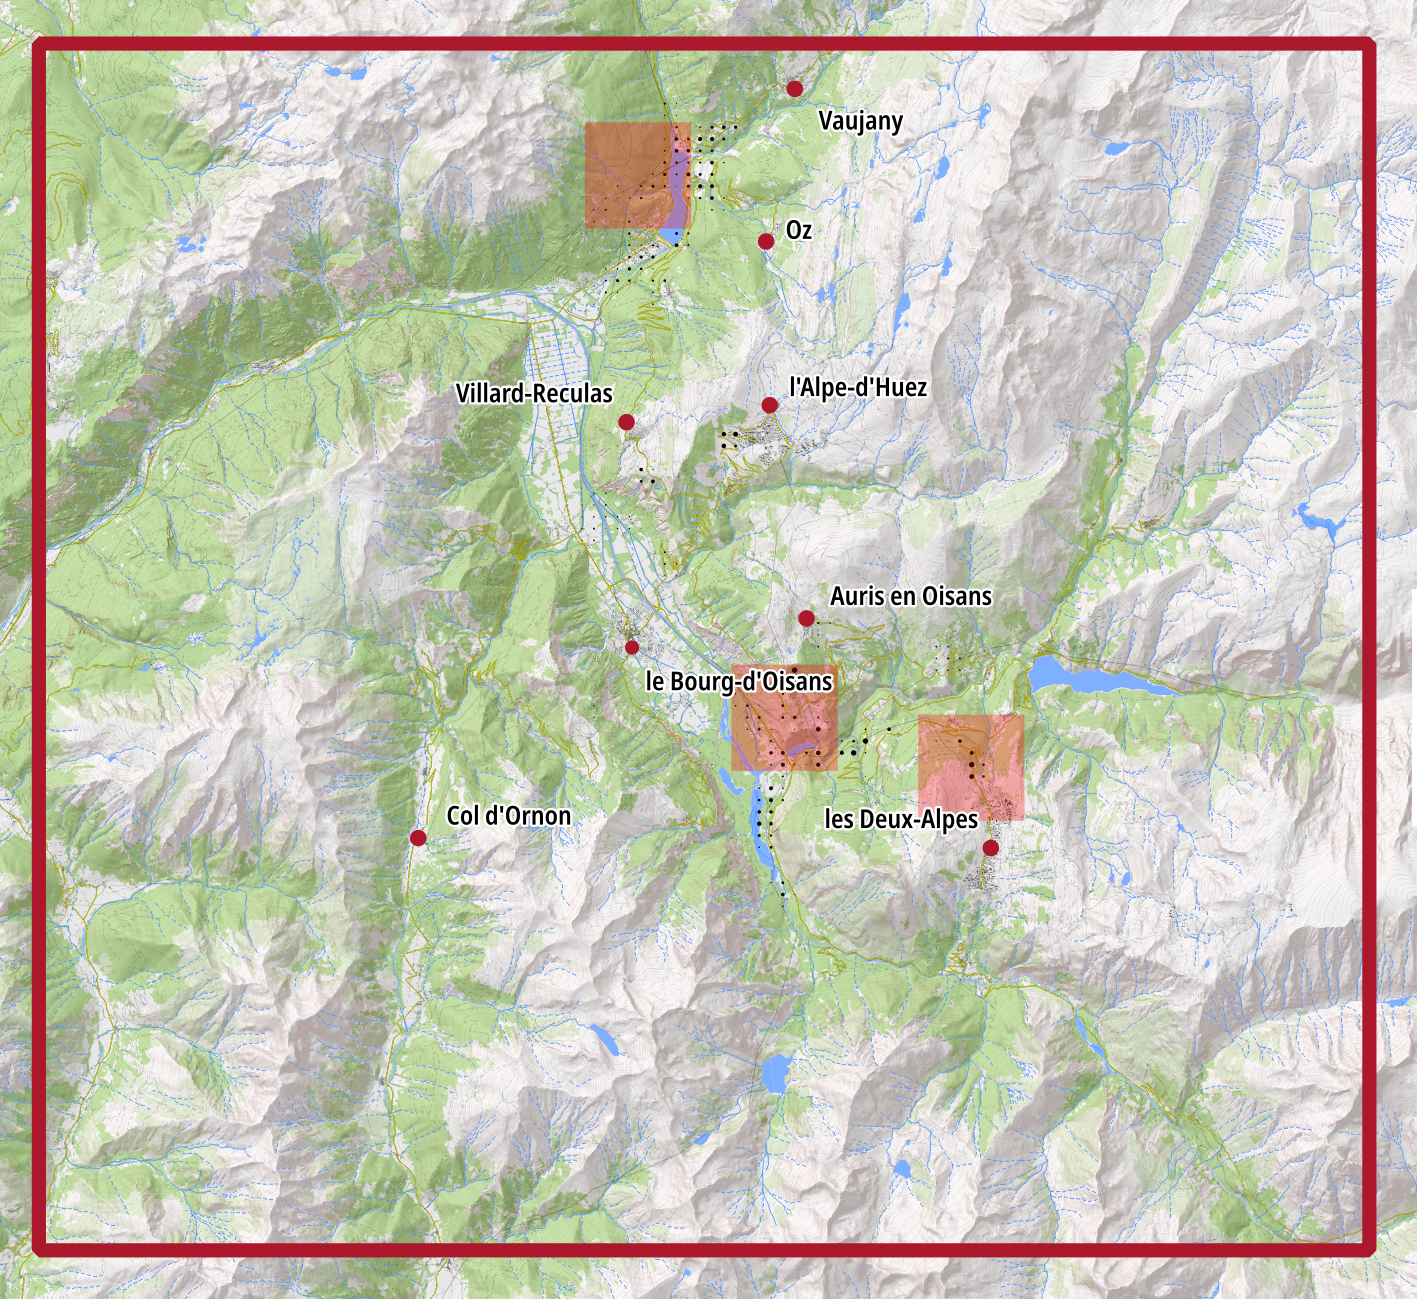
\includegraphics{../figures/ZLP_V2_FilRouge/ZLP.png}};
    \begin{scope}
      \node (P2) at ([yshift=-.5cm]img.south east) {};
      \node (P1) at ([yshift=-.5cm]img.south west) {};
      % 
      \node (rect) [anchor=north west, minimum width=1cm,minimum
      height=.25cm] at ([yshift=-.25cm]P1) {}; \path[draw=RdBu-9-1, line
      width=1mm](rect.west) --([xshift=-1ex]rect.south) -- ([xshift=1ex]rect.north)
      -- (rect.east);
      % 
      \node[anchor=west, font=\tiny\vphantom{Ag}, text width = 4cm] at
      ([xshift=1ex]rect.east) {Limite de la \ac{zir}};
      % 
      \node[anchor=west, font=\footnotesize\vphantom{Ag}] at
      (P1 |- 0cm,-1.7cm) {Degré d'appartenance :};
      % 
      \begin{scope}
        \foreach \x [evaluate=\xshift using 1+\x/10, evaluate=\rad using (\x * .0004) + .01] in {0,...,100}
        {
          \draw[fill=black,draw=none, below] ([xshift=\xshift cm, yshift=-2cm]P1) circle [radius=\rad cm];
        }
        % 
        \path(1,-2.5) --++ (10,0)
        node[et,pos=0] {0}
        node[et,pos=.5] {0,5}
        node[et,pos=1] {1};
      \end{scope}
      % Échelle
      \draw[-] (P2 |- -1cm,-1cm) --++ (-1,0) node[et,pos=.5] {\SI{2,5}{\kilo\meter}};
      % Légende détaillée
      \path (P1) -- (P2) node[pos=.5, yshift=-2.5cm] {\tiny Pour la légende détaillée du fond topographique voir \autoref{anx:topo_leg}. Sources: BD TOPO 2018, BD ALTI 2018.}; 
    \end{scope}
    \begin{scope}[x=(img.south east),y=(img.north west)]
      \node[draw,RdBu-9-1,thick,minimum height=1.6cm,minimum width=1.00cm] (B1) at (0.2,0.60) {};
      \node[draw,RdBu-9-1,thick,minimum height=0.8cm,minimum width=0.50cm] (B2) at (0.7,0.25) {};
      \node[draw,RdBu-9-1,thick,minimum height=0.4cm,minimum width=0.25cm] (B3) at (0.9,0.10) {};
    \end{scope}
  \end{tikzpicture}
}

\subfloat[\label{fig:zlp_fil_rouge_a}]{%
  \begin{tikzpicture}[remember picture,inner sep=0pt,outer sep=0pt]
    \tikzset{et/.style={above,font=\footnotesize\vphantom{Ag}}}
    \node (img1)
    {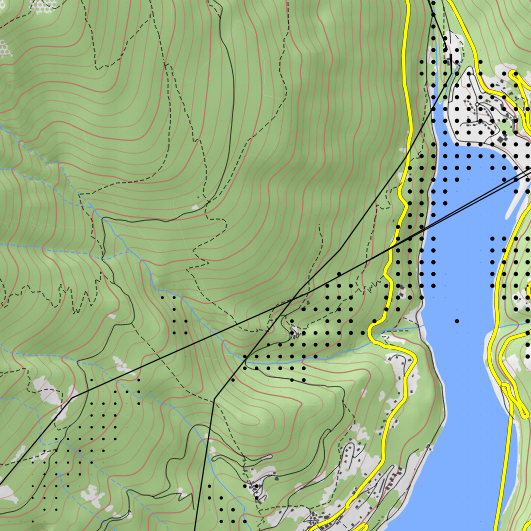
\includegraphics{../figures/ZLP_V2_FilRouge/ZLP_3.png}};
    \draw[-] ([yshift=-1cm]img1.south east) --++ (-1,0) node[et,pos=.5] {\SI{500}{\meter}};
    \draw[RdBu-9-1,thick,draw] (img1.south west) rectangle (img1.north east);
  \end{tikzpicture}
}\hfill
% 
\subfloat[\label{fig:zlp_fil_rouge_b}]{%
  \begin{tikzpicture}[remember picture,inner sep=0pt,outer sep=0pt]
    \tikzset{et/.style={above,font=\footnotesize\vphantom{Ag}}}
    \node (img2)
    {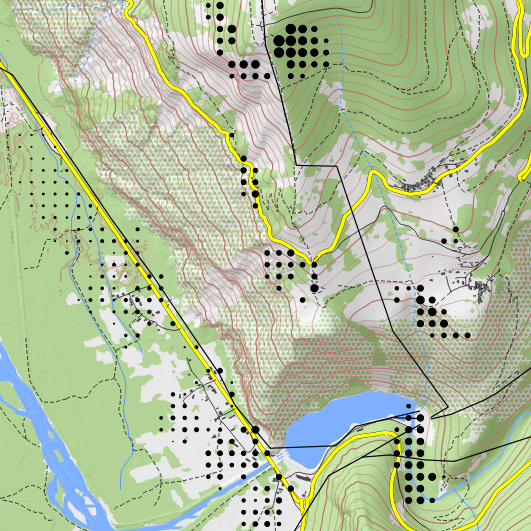
\includegraphics{../figures/ZLP_V2_FilRouge/ZLP_2.png}};
    \draw[-] ([yshift=-1cm]img2.south east) --++ (-1,0) node[et,pos=.5] {\SI{500}{\meter}};
    \draw[RdBu-9-1,thick,draw] (img2.south west) rectangle (img2.north east);
  \end{tikzpicture}
}\hfill
% 
\subfloat[\label{fig:zlp_fil_rouge_c}]{%
  \begin{tikzpicture}[remember picture,inner sep=0pt,outer sep=0pt]
    \tikzset{et/.style={above,font=\footnotesize\vphantom{Ag}}}
    \node (img3)
    {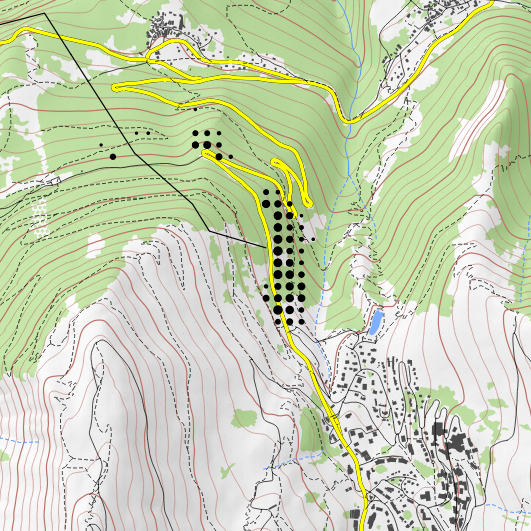
\includegraphics{../figures/ZLP_V2_FilRouge/ZLP_4.png}};
    \draw[-] ([yshift=-1cm]img3.south east) --++ (-1,0) node[et,pos=.5] {\SI{500}{\meter}};
    \draw[RdBu-9-1,thick,draw] (img3.south west) rectangle (img3.north east);
  \end{tikzpicture}
}
\begin{tikzpicture}[overlay, remember picture,RdBu-9-1,thick,draw,inner sep=0pt,outer sep=0pt]
  \draw (B1) -- (img1);
  \draw (B2) -- (img2);
  \draw (B3) -- (img3);
\end{tikzpicture}
  \caption{\ac{zlp} de l'alerte \emph{fil rouge}}
  \label{fig:zlp_fil_rouge}
\end{figure}


\subsection{Critique de la modélisation}
\label{subsec:9-4-3}

%%% Local Variables:
%%% mode: latex
%%% TeX-master: "../../../../main"
%%% End:
